\documentclass[12pt]{article}
\usepackage[spanish]{babel}
\selectlanguage{spanish}
\usepackage[utf8]{inputenc}
\usepackage{vmargin}
\usepackage{graphicx}
\setmargins{2.3cm}{1.3cm}{16.5cm}{23.2cm}{0pt}{1cm}{0pt}{2cm}
\title{Usando Gnuplot}
\author{Jesús Valenzuela Nieblas}
\date{}

\begin{document}
\maketitle
\section{Introducción}
En cálculo, el teorema de Taylor, recibe su nombre del matemático británico Brook Taylor, quien lo enunció con mayor generalidad en 1712, aunque previamente James Gregory lo había descubierto en 1671. Este teorema permite obtener aproximaciones polinómicas de una función en un entorno de cierto punto en que la función sea diferenciable. Además el teorema permite acotar el error obtenido mediante dicha estimación.

El Teorema de Taylor Nos dice que : sea f continua en [a, b] y con derivadas hasta de orden n continuas también en este intervalo cerrado; supóngase que f (n+1) (x) existe en (a,b), entonces para x y xoÎ (a,b) se tiene: $(a,x)$, entonces se cumple que:

$$ P_T(x)= f(x_o)+f'(x_o)(x-x_o)+ {f^{(2)}(x_o)\over 2!}(x-x_o)^2+\cdots+{f^{(n)}(x_o)\over n!}(x-x_o)^n+E_n $$
Donde:
$$ E_n={f^{(n+1)}(c)\over (n+1) !}(x-x_o)^{n+1} $$




\subsection{Aproximación de Taylor la función $Sin(x)$}
Se utilizó el siguiente código en máxima

\begin{verbatim}

/* [wxMaxima batch file version 1] [ DO NOT EDIT BY HAND! ]*/
/* [ Created with http://maxima-online.org ] */

/* [wxMaxima: comment start ]
This solution online http://maxima-online.org/?inc=r1843860752
   [wxMaxima: comment end   ] */

/* [wxMaxima: input   start ] */
f(x):= sin(x);
P1(x):=taylor(f(x), x, 0, 1);
P3(x):=taylor(f(x), x, 0, 3);
P5(x):=taylor(f(x), x, 0, 5);
P7(x):=taylor(f(x), x, 0, 7);
fortran(P1(x));
fortran(P3(x));
fortran(P5(x));
fortran(P7(x));
tex(P1(x));
tex(P3(x));
tex(P5(x));
tex(P7(x));
 plot2d ([f(x),P1(x), P3(x), P5(x), P7(x)], [x, -%pi, %pi], [y, -2, 2],[style,[lines,3],[xlabel, "X"], [ylabel, "Y"]], [color,red,green,blue,magenta,cyan],  [legend,"y=sin(x)","y=P1(x)","y=P3(x)","y=P5(x)", "y=P7(x)"], [axes, true], [box,false]);
/* [wxMaxima: input   end   ] */
\end{verbatim}

Y nos dió como resultado ésta gráfica
\begin{center}
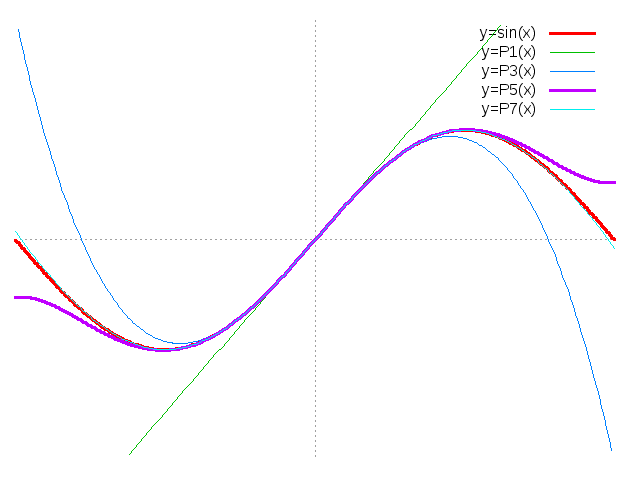
\includegraphics[scale=.5]{sin.png}
\end{center}
\pagebreak
\subsection{Aproximación de Taylor de la función $log(1+x)$}
Se desarrollo el siguiente código
\begin{verbatim}
/* [wxMaxima batch file version 1] [ DO NOT EDIT BY HAND! ]*/
/* [ Created with http://maxima-online.org ] */

/* [wxMaxima: comment start ]
This solution online http://maxima-online.org/?inc=r-1564318875
   [wxMaxima: comment end   ] */

/* [wxMaxima: input   start ] */
f(x):= log(1+x);
T4(x):=taylor(f(x), x, 0, 4);
T7(x):=taylor(f(x), x, 0, 7);
T11(x):=taylor(f(x), x, 0, 11);
T16(x):=taylor(f(x), x, 0, 16);
fortran(T4(x));
fortran(T7(x));
fortran(T11(x));
fortran(T16(x));
tex(T4(x));
tex(T7(x));
tex(T11(x));
tex(T16(x));
plot2d ([f(x),T4(x), T7(x), T11(x), T16(x)], [x, -1.5, 1.5], [y, -4, 2], [color,pink,green,red,orange,blue],[legend, "log(1+x)", "P4", "P7", "P11", "P16"],[axes, true]);
/* [wxMaxima: input   end   ] */

\end{verbatim}

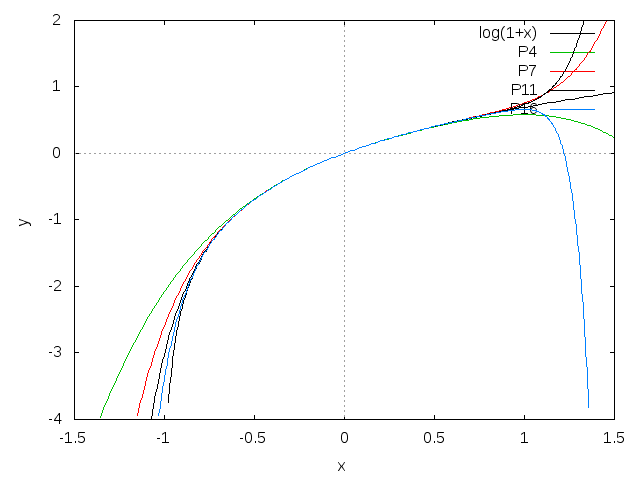
\includegraphics[scale=.5]{log1+x.png}
\begin{center}

\end{center}
\pagebreak
\subsection{Aproximación de Taylor la función  $log(cos(x))$}

\begin{verbatim}
/* [wxMaxima batch file version 1] [ DO NOT EDIT BY HAND! ]*/
/* [ Created with http://maxima-online.org ] */

/* [wxMaxima: comment start ]
This solution online http://maxima-online.org/?inc=r1484266984
   [wxMaxima: comment end   ] */

/* [wxMaxima: input   start ] */
f(x):= log(cos(x));
T3(x):=taylor(f(x), x, 0, 3);
T6(x):=taylor(f(x), x, 0, 6);
T9(x):=taylor(f(x), x, 0, 9);
T12(x):=taylor(f(x), x, 0, 12);
fortran(T3(x));
fortran(T6(x));
fortran(T9(x));
fortran(T12(x));
tex(T3(x));
tex(T6(x));
tex(T9(x));
tex(T12(x));
plot2d ([f(x),T3(x),T6(x),T9(x),T12(x)],[x, -%pi/2, %pi/2],[y, -4, 2],[legend, "log(cos)", "T3", "T6", "T9", "T12"],[style,[lines,2]]);
/* [wxMaxima: input   end   ] */

\end{verbatim}


\begin{center}
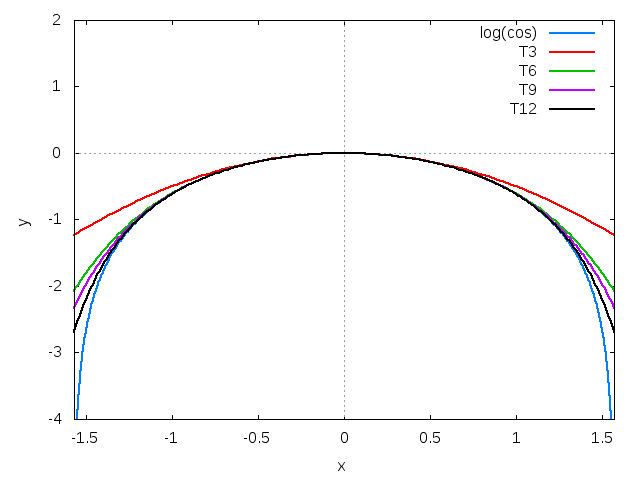
\includegraphics[scale=.5]{logcos.png}
\end{center}
\pagebreak
\subsection{Aproximación de  Taylor de la función $ e^x \over cos(x)$}

\begin{verbatim}
/* [wxMaxima batch file version 1] [ DO NOT EDIT BY HAND! ]*/
/* [ Created with http://maxima-online.org ] */

/* [wxMaxima: comment start ]
This solution online http://maxima-online.org/?inc=r-354090405
   [wxMaxima: comment end   ] */

/* [wxMaxima: input   start ] */
f(x):= exp(x)/cos(x);
T3(x):=taylor(f(x), x, 0, 3);
T6(x):=taylor(f(x), x, 0, 6);
T9(x):=taylor(f(x), x, 0, 9);
T12(x):=taylor(f(x), x, 0, 12);
fortran(T3(x));
fortran(T6(x));
fortran(T9(x));
fortran(T12(x));
tex(T3(x));
tex(T6(x));
tex(T9(x));
tex(T12(x));
plot2d ([f(x),T3(x),T6(x),T9(x),T12(x)],[x, -%pi/2, %pi/2],[y, -4, 2],[legend, "exp(x)/cos(x)", "T3", "T6", "T9", "T12"],[style,[lines,2]]);
/* [wxMaxima: input   end   ] */

\end{verbatim}


\begin{center}
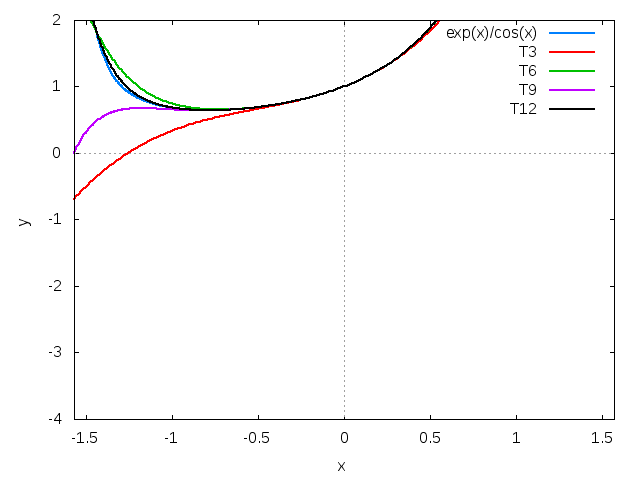
\includegraphics[scale=.5]{expcos.png}
\end{center}
\pagebreak
\subsection{Aproximación de Taylorde la función $e^x(x+1)$}

\begin{verbatim}
/* [wxMaxima batch file version 1] [ DO NOT EDIT BY HAND! ]*/
/* [ Created with http://maxima-online.org ] */

/* [wxMaxima: comment start ]
This solution online http://maxima-online.org/?inc=r-445163449
   [wxMaxima: comment end   ] */

/* [wxMaxima: input   start ] */
f(x):= (1+x)*exp(x);
T3(x):=taylor(f(x), x, 0, 3);
T6(x):=taylor(f(x), x, 0, 6);
T9(x):=taylor(f(x), x, 0, 9);
T12(x):=taylor(f(x), x, 0, 12);
fortran(T3(x));
fortran(T6(x));
fortran(T9(x));
fortran(T12(x));
tex(T3(x));
tex(T6(x));
tex(T9(x));
tex(T12(x));
plot2d ([f(x),T3(x),T6(x),T9(x),T12(x)],[x, -5, 5],[y, -10, 10],[legend, "(1+x)*exp(x)", "T3", "T6", "T9", "T12"],[style,[lines,2]]);
/* [wxMaxima: input   end   ] */

\end{verbatim}

\begin{center}
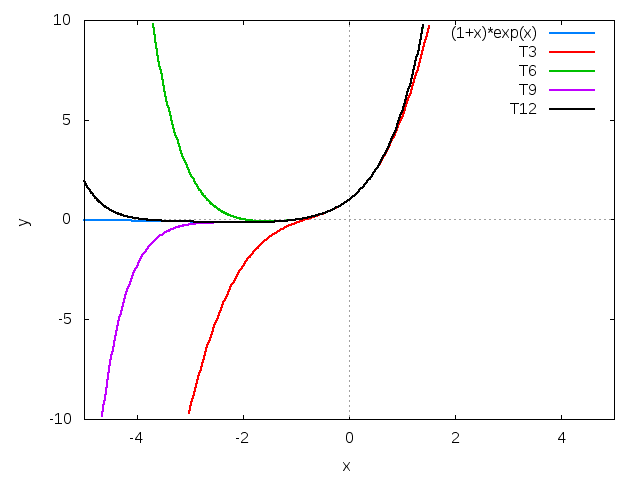
\includegraphics[scale=.5]{1xexp.png}
\end{center}
\end{document}
